\documentclass[answers]{exam}
\usepackage{../../mypackages}
\usepackage{../../macros}

%\usepackage{blindtext}

\SolutionEmphasis{\color{blue}}
\renewcommand{\solutiontitle}{\noindent}

\renewcommand{\arraystretch}{1.5} % Augmente l'espacement vertical entre les lignes du tableau
\newcolumntype{C}{>{\centering\arraybackslash}m{2cm}}

\SetLabelAlign{myright}{\hss\llap{$#1$}}
\newlist{where}{description}{1}
\setlist[where]{labelwidth=2cm,labelsep=1em,
                        leftmargin=!,align=myright,font=\normalfont}

\setlength{\parindent}{0pt}

\title{Interrogation N° 3 - Frises / Sections / Géométrie}
\author{N. Bancel}
\date{5 Février 2025}

\begin{document}


\textbf{Collège Lycée Suger}
\hfill
\textbf{Mathématiques} \\

\textbf{Année 2024-2025}
\hfill
\textbf{1ères STD2A} \par

{\let\newpage\relax\maketitle}
%\maketitle

  
  {\let\newpage\relax\maketitle}

  \begin{center}
  \textbf{\textcolor{red}{Durée : 45 minutes. La calculatrice n'est pas autorisée}} \\
  \textbf{\textcolor{red}{Une réponse donnée sans justification sera considérée comme fausse.}} \\
  Cette interrogation contient \numquestions\ questions, sur \numpages\ pages et est notée sur 20 points. 
  
  \end{center}

\section*{Exercice 1 - Frises et figures régulières (3 points)}

\begin{questions}
\question[3] (1.5 points par figure) Pour chacune des frises ci-dessous : (1) repérer le motif. (2) tracer le vecteur permettant de construire la frise à partir du motif.
\begin{figure}[H]
  \centering
  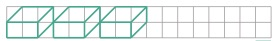
\includegraphics[width=0.5\linewidth]{img/interro_03_01.jpg}
\end{figure}
\begin{figure}[H]
  \centering
  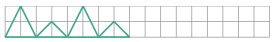
\includegraphics[width=0.5\linewidth]{img/interro_03_02.jpg}
\end{figure}
\end{questions}

\section*{Exercice 2 - Transformations (5 points)}
\begin{questions}
\question[2] Construire le centre E qui transforme la figure verte en la figure rouge par symétrie centrale. Vérifier qu'il "fonctionne" pour chaque point.
\begin{figure}[H]
  \centering
  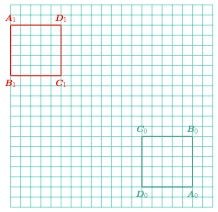
\includegraphics[width=0.5\linewidth]{img/interro_03_04.jpg}
\end{figure}

\question[3] Construire la rotation de centre E et d'angle $135°$ (sens horaire) pour la figure suivante.

\begin{figure}[H]
  \centering
  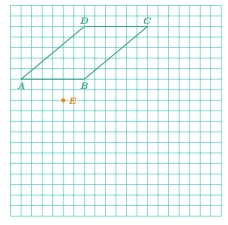
\includegraphics[width=0.5\linewidth]{img/interro_03_05.jpg}
\end{figure}
\end{questions}

\section*{Exercice 2 - Polygones réguliers (4 points)}

\begin{questions}
  \question[1] Quelles sont les propriétés d'un polygône régulier ?
  \question[3] Construire un octogone régulier.
\end{questions}

\section*{Exercice 3 - Pavage (8 points)}

\begin{figure}[H]
  \centering
  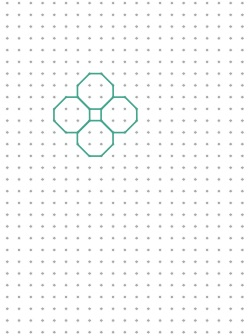
\includegraphics[width=0.5\linewidth]{img/interro_03_03.jpg}
  \captionsetup{labelformat=empty}
  \caption{\label{} Pavage}
\end{figure}

\begin{questions}
  \question[1] Repérer la maille élémentaire du motif donné 
  \question[3] Par quelles transformations obtient-on le motif à partir de la maille élémentaire ?
  \question[2] Compléter la figure suivante afin de réaliser un pavage (vous pouvez dessiner le motif ~5 fois de plus)
  \question[2] Tracer les deux vecteurs permettant de créer ce pavage par translation du motif donné.
\end{questions}


\end{document}
